%!TEX root =  cpt-rl-icml.tex
We consider a traffic signal control application where the aim is to improve the road user experience by an adaptive traffic light control (TLC) algorithm.
We apply the CPT-functional to the delay experienced by road users, since CPT realistically captures the attitude of the road users towards delays. We then optimize the CPT-value of the delay and contrast this approach with traditional expected delay optimizing algorithms. It is assumed that the CPT functional's parameters $(u,w)$ are given (usually, these are obtained by observing human behavior). The experiments are performed using the GLD traffic simulator \cite{GLDSim} and the implementation is available at \url{https://bitbucket.org/prashla/rl-gld}.

%\paragraph{Simulation Setup:}  
We consider a road network with $\N$ signalled lanes that are spread across junctions and $\M$ paths, where each path connects (uniquely) two edge nodes, from which the traffic is generated -- cf. \cref{fig:2x2grid}. 
%\todoc{Can we have a higher quality figure?}
At any instant $n$, let $q_n^i$ and $t_n^i$ denote the queue length and elapsed time since the lane turned red, for any lane $i = 1,\ldots, \N$. Let $d_n^{i,j}$ denote the delay experienced by $j$th road user on $i$th path, for any $i=1,\ldots,\M$ and $j=1,\ldots,n_i$, where $n_i$ denotes the number of road users on path $i$.
We specify the various components of the traffic control MDP below.
The state $s_n=(q_n^1,\ldots,q_n^{\N},t_n^1,\ldots,t_n^{\N},d_n^{1,1},\ldots,d_n^{\M,n_{\M}})\tr$ is a vector of lane-wise queue lengths, elapsed times and pathwise delays.
The actions are the feasible traffic signal configurations. 

We consider three different notions of return as follows:
%
\textbf{CPT:} Let $\mu^i$ be the proportion of road users along path $i$, for $i=1,\ldots,\M$. Any road user along path $i$ will evaluate the delay he experiences in a manner that is captured well by CPT. Let $X_i$ be the delay r.v. for path $i$ and let the corresponding CPT-value be $\C(X_i)$. With the objective of maximizing the experience of road users across paths, the overall return to be optimized is given by
\begin{align}
\text{CPT}(X_1,\ldots,X_{\M}) = \sum_{i=1}^{\M} \mu^i \C(X_i).\label{eq:cpt-traffic}
\end{align}
% \textbf{EUT:} Here we only use the utility functions $u^+$ and $u^-$ to handle gains and losses, but do not distort probabilities. 
% Thus, the EUT objective is defined as
% \begin{align*}
% \text{EUT}(X_1,\ldots,X_{\M}) = \sum_{i=1}^{\M} \mu^i \left(\E(u^+(X_i) - \E(u^-(X_i)\right),
% \end{align*}
% where $\E(u^+(X_i)) = \intinfinity \Prob{u^+(X_i)>z} dz$ and $\E(u^-(X_i)) - \intinfinity \Prob{u^-(X_i)>z} dz$, for $i=1,\ldots,\M$.

\textbf{AVG:} This is the usual expected value with no distinction between gains and losses via utility functions and no distortion of probabilities, i.e.,\\[1ex] 
\centerline{$\text{AVG}(X_1,\ldots,X_{\M}) = \sum_{i=1}^{\M} \mu^i \E(X_i).$} 
%Thus, the AVG objective is defined as
%\begin{align}
%\text{AVG}(X_1,\ldots,X_{\M}) = \sum_{i=1}^{\M} \mu^i \E(X_i).
%\end{align}   
%where $\E(X_i) = \intinfinity P(u^+(X_i)>z) dz - \intinfinity P(u^-(X_i)>z) dz$.

An important component of CPT is to employ a reference point to calculate gains and losses. 
%Choosing a suitable reference point is challenging, but \cite{tversky1992advances} advocate using status-quo as the reference point. 
In our setting, we use path-wise delays obtained from a pre-timed TLC (cf. the Fixed TLCs in \cite{prashanth2011reinforcement}) as the reference point. If the delay of any algorithm (say CPT-SPSA) is less than that of pre-timed TLC, then the (positive) difference in delays is perceived as a gain and in the complementary case, the delay difference is perceived as a loss. Thus, the CPT-value $\C(X_i)$ for any path $i$ in \eqref{eq:cpt-traffic} is to be understood as a \textit{differential delay}.  

%, as the road network considered is high-dimensional (state space cardinality $> 10^{60}$). 

Using a Boltzmann policy that has the form
$$
\pi_{\theta}(s,a) = \frac{e^{\theta^{\top} \phi_{s,a}}}{\sum_{a' \in {\A(s)}} e^{\theta^{\top} \phi_{s,a'}}},
\hspace{6pt} \forall s \in \S,\;\forall a \in \A(s),
$$
with features $\phi_{s,a}$ as described in Section V-B of \cite{prashanth2012threshold},
we implement the following TLC algorithms:

{\bf\em CPT-SPSA}: This is the first-order algorithm with SPSA-based gradient estimates, as described in Algorithm \ref{alg:1spsa}. In particular, the estimation scheme in Algorithm \ref{alg:holder-est} is invoked to estimate $\C(X_i)$ for each path $i=1,\ldots,\M$, with $d_n^{i,j}, j=1,\ldots,n_i$ as the samples.

% {\bf\em EUT-SPSA}: This is similar to CPT-SPSA, except that weight functions $w^+(p)=w^-(p)=p,$ for $p\in [0,1]$. 

{\bf\em AVG-SPSA}: This is similar to CPT-SPSA, except that the underlying SPSA algorithm uses average delays for each path for performing the descent. 

For both CPT-SPSA, we set the utility functions (see \eqref{eq:cpt-general}) as follows:
$$u^+(x) =  |x|^{\sigma}, \text{ and  }u^-(x) = \lambda |x|^{\sigma},$$ 
where $\lambda = 2.25$ and $\sigma = 0.88$.
For CPT-SPSA, we set the weights as follows:
\begin{align*}
w^+(p) &= \frac{p^{\eta_1}}{{(p^{\eta_1}+ (1-p)^{\eta_1})}^{\frac{1}{\eta_1}}}, \text{ and }\\  
w^-(p) &= \frac{p^{\eta_2}}{{(p^{\eta_2}+ (1-p)^{\eta_2})}^{\frac{1}{\eta_2}}},
\end{align*} 
where $\eta_1 = 0.61$ and $\eta_2 = 0.69$. The choices for $\lambda$, $\sigma$, $\eta_1$ and $\eta_2$ are based on median estimates given by \cite{tversky1992advances} and have been used earlier in a traffic application (see \cite{gao2010adaptive}).
For all the algorithms,
 motivated by standard guidelines (see \cite{spall2005introduction}),
 we set $\delta_n = 1.9/n^{0.101}$ and $a_n = 1/(n+50)$. The initial point $\theta_0$ is the $d$-dimensional vector of ones and $\forall i$, the operator $\Gamma_i$ keeps the iterate $\theta_i$ bounded within $[0.1, 1.0]$.
    
The experiments involve two phases:
first, a training phase where we run each algorithm for $200$ iterations, with each iteration involving two perturbed simulations, each of trajectory length $500$. This is followed by a test phase where we fix the policy for each algorithm and $100$ independent simulations of the MDP (each with a trajectory length of $1000$) are performed. After each run in the test phase, the overall CPT-value \eqref{eq:cpt-traffic} is estimated. 
%\paragraph{Results:} 

Figures \ref{fig:avg}--\ref{fig:cpt} present the histogram of the CPT-values from the test phase for AVG-SPSA and CPT-SPSA, respectively.  A similar exercise for pre-timed TLC resulted in a CPT-value of $-46.14$. It is evident that each algorithm converges to a different policy. However, the CPT-value of the resulting policies is highest in the case of CPT-SPSA. Intuitively, this is expected because AVG-SPSA uses neither utilities nor probability distortions.
The results in Figure \ref{fig:histogram-perf} argue for specialized algorithms that incorporate CPT-based criteria, esp. in the light of previous findings which show CPT matches human evaluation well and there is a need for algorithms that serve human needs well.
%\todoc{It would be nice to point out how the CPT policy is different than the others.}

 %\begin{figure}
    %\centering
        %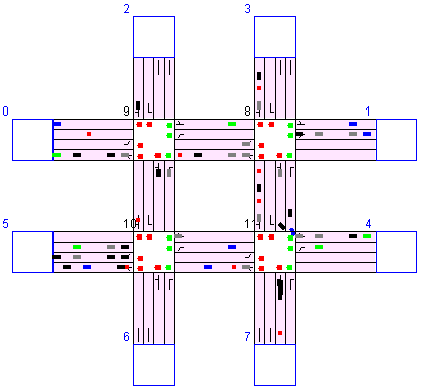
\includegraphics[width=2in, height=1.2in]{fig/2x2grid.png}
%\caption{Snapshot of a 2x2-grid network from GLD simulator. The figure shows eight edge nodes that generate traffic, four traffic lights and twelve four-laned roads carrying cars.}
%\label{fig:2x2grid}
%\end{figure}


 \begin{figure}

%\vspace{-2.5ex}

    \centering
     \begin{tabular}{c}
\subfigure[Snapshot of a 2x2-grid network from GLD simulator. The figure shows eight edge nodes that generate traffic, four traffic lights and  four-laned roads carrying cars. ]{
\label{fig:2x2grid}
        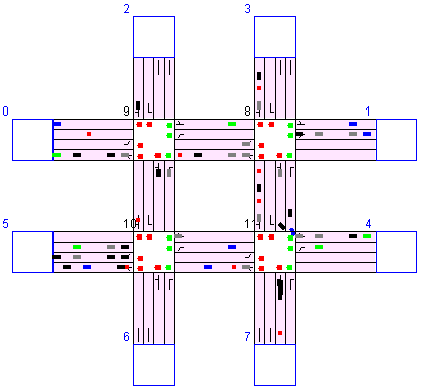
\includegraphics[width=2in,height=1.5in]{fig/2x2grid.png}
}
\\		
\subfigure[AVG-SPSA]{
\label{fig:avg}
%\hspace{2em} 
\tabl{c}{\scalebox{0.72}{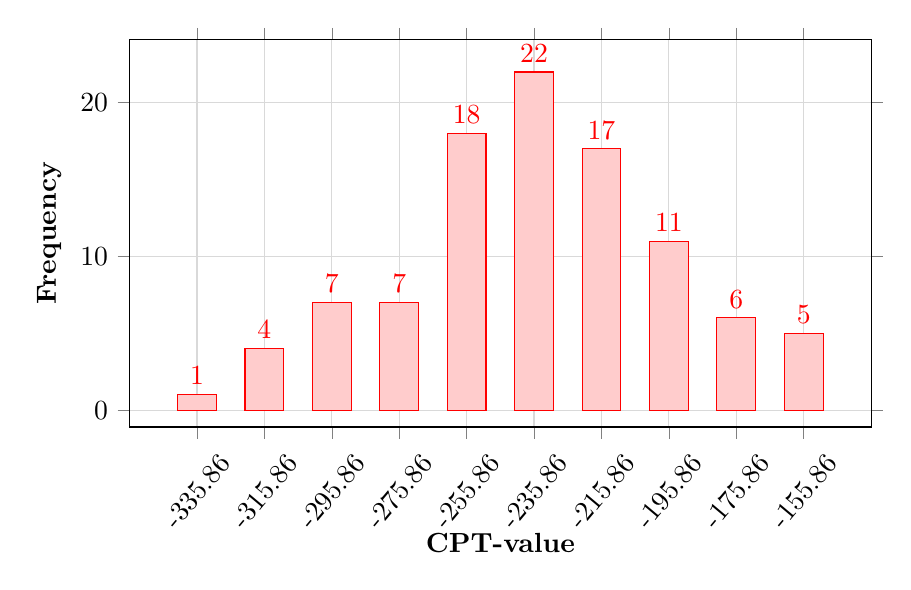
\begin{tikzpicture}
\begin{axis}[
ybar={2pt},
%  legend style={at={(0.5,-0.2)},anchor=north,legend columns=-1},
legend pos=outer north east,
legend image code/.code={\path[fill=white,white] (-2mm,-2mm) rectangle
(-3mm,2mm); \path[fill=white,white] (-2mm,-2mm) rectangle (2mm,-3mm); \draw
(-2mm,-2mm) rectangle (2mm,2mm);},
ylabel={\bf Frequency},
xlabel={\textbf{CPT-value}},
x label style={at={(axis description cs:0.5,-0.25)},anchor=north},
symbolic x coords={0, -335.86, -315.86, -295.86, -275.86, -255.86, -235.86, -215.86, -195.86, -175.86, -155.86, 11},
xmin={0},
xmax={11},
xtick=data,
ytick align=outside,
%xticklabels={{\bf7x9-Grid\\[0.5ex]($d=504$),\bf 14x9-Grid\\[0.5ex]($d=1008$),\bf 14x18-Grid\\[0.5ex]($d=2016$),\bf 28x18-Grid\\[0.5ex]($d=4032$)}},
xticklabel style={rotate=50, align=center},
bar width=14pt,
nodes near coords,
grid,
grid style={gray!30},
width=11cm,
height=6.5cm,
]
\addplot[red, fill=red!20]   coordinates {  (-335.86,1) (-315.86,4) (-295.86,7) (-275.86,7) (-255.86,18) (-235.86,22) (-215.86,17) (-195.86,11) (-175.86,6) (-155.86,5)}; %LSPI
\end{axis}
\end{tikzpicture}}\\[1ex]}
}
\\
%%%%%%%%%%%%%%
\subfigure[EUT-SPSA]{
\label{fig:eut}
%\hspace{2em} 
\tabl{c}{\scalebox{0.72}{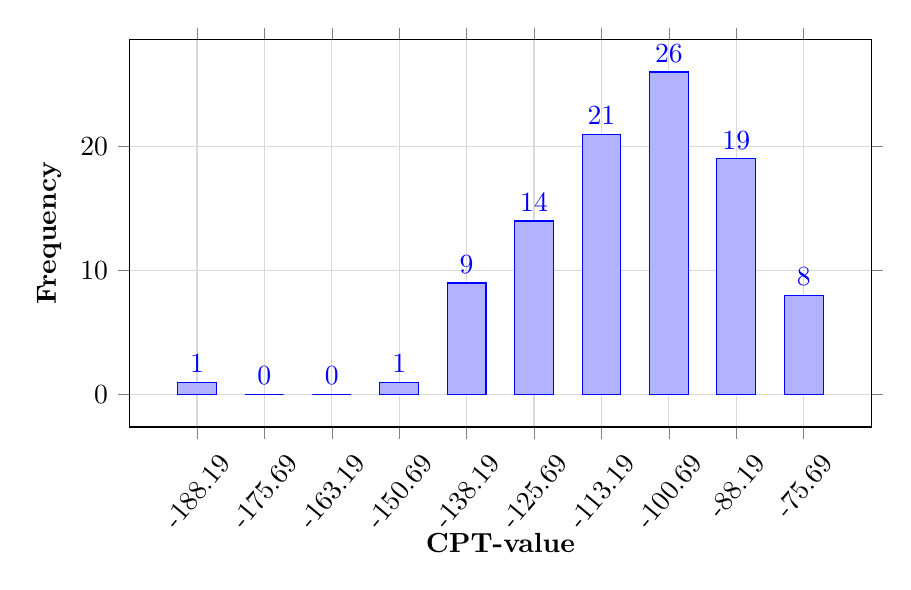
\begin{tikzpicture}
\begin{axis}[
ybar={2pt},
%  legend style={at={(0.5,-0.2)},anchor=north,legend columns=-1},
legend pos=outer north east,
legend image code/.code={\path[fill=white,white] (-2mm,-2mm) rectangle
(-3mm,2mm); \path[fill=white,white] (-2mm,-2mm) rectangle (2mm,-3mm); \draw
(-2mm,-2mm) rectangle (2mm,2mm);},
ylabel={\bf Frequency},
xlabel={\textbf{CPT-value}},
x label style={at={(axis description cs:0.5,-0.25)},anchor=north},
symbolic x coords={0,-188.19,-175.69,-163.19,-150.69,-138.19,-125.69,-113.19,-100.69,-88.19,-75.69,11},
xmin={0},
xmax={11},
xtick=data,
ytick align=outside,
%xticklabels={{\bf7x9-Grid\\[0.5ex]($d=504$),\bf 14x9-Grid\\[0.5ex]($d=1008$),\bf 14x18-Grid\\[0.5ex]($d=2016$),\bf 28x18-Grid\\[0.5ex]($d=4032$)}},
xticklabel style={rotate=50, align=center},
bar width=14pt,
nodes near coords,
grid,
grid style={gray!30},
width=11cm,
height=6.5cm,
]
\addplot   coordinates {  (-188.19,1) (-175.69,0) (-163.19,0) (-150.69,1) (-138.19,9) (-125.69,14) (-113.19,21) (-100.69,26) (-88.19,19) (-75.69,8) }; %LSPI
\end{axis}
\end{tikzpicture}}\\[1ex]}
}
\\
%%%%%%%%%%%%%%%%%%%%%%%%%
\subfigure[CPT-SPSA]{
\label{fig:cpt}
%\hspace{2em} 
\tabl{c}{\scalebox{0.72}{\begin{tikzpicture}
\begin{axis}[
ybar={2pt},
%  legend style={at={(0.5,-0.2)},anchor=north,legend columns=-1},
legend pos=outer north east,
legend image code/.code={\path[fill=white,white] (-2mm,-2mm) rectangle
(-3mm,2mm); \path[fill=white,white] (-2mm,-2mm) rectangle (2mm,-3mm); \draw
(-2mm,-2mm) rectangle (2mm,2mm);},
ylabel={\bf Frequency},
xlabel={\textbf{CPT-value}},
x label style={at={(axis description cs:0.5,-0.22)},anchor=north},
symbolic x coords={0, -43.36,-33.36,-23.36,-13.36,-3.36,6.64,16.64,26.64,36.64,46.64, 11},
xmin={0},
xmax={11},
xtick=data,
ytick align=outside,
%xticklabels={{\bf7x9-Grid\\[0.5ex]($d=504$),\bf 14x9-Grid\\[0.5ex]($d=1008$),\bf 14x18-Grid\\[0.5ex]($d=2016$),\bf 28x18-Grid\\[0.5ex]($d=4032$)}},
xticklabel style={rotate=50, align=center},
bar width=14pt,
nodes near coords,
grid,
grid style={gray!30},
width=11cm,
height=6.5cm,
]
\addplot[darkgreen, fill=darkgreen!20]   coordinates {  (-43.36,1) (-33.36,0) (-23.36,0) (-13.36,1) (-3.36,0) (6.64,1) (16.64,8) (26.64,52) (36.64,24) (46.64,12) }; %LSPI
\end{axis}
\end{tikzpicture}}\\[1ex]}
}
\end{tabular}
\caption{Histogram of CPT-value of the differential delay (calculated with a pre-timed TLC as reference point) for three different algorithms (all based on SPSA): AVG uses plain sample means (no utility/weights), EUT uses utilities but no weights and CPT uses both utilites and weights. Note: larger values are better.}
\label{fig:histogram-perf}
\end{figure}
